\documentclass[12pt,a4paper]{article}
\usepackage[utf8]{inputenc}
\usepackage{amsmath}
\usepackage{listings}
\usepackage{verbatim}
\usepackage{graphicx} 
\oddsidemargin 0cm
\marginparwidth 0cm
\hoffset 0cm
\usepackage{polski}
\begin{document} 
\large
\begin{tabular}{|c|c|c|c|}
\hline
\multicolumn{4}{|l|}{Temat:}\\
\multicolumn{4}{|c|}{Poszukiwanie minimum wartości funkcji w~dwóch wymiarach}\\
\multicolumn{4}{|c|}{metodą Newtona}\\
\hline
\multicolumn{1}{|l}{Wykonał:}&\multicolumn{1}{|l}{Wydział:}&\multicolumn{1}{|c}{Kierunek}&\multicolumn{1}{|l|}{Grupa:}\\
Marcin Fabrykowski&FiIS&Inf. Stos.&grupa 3\\
\hline
\end{tabular}
\normalsize
\vspace{2cm}
\begin{enumerate}
\item Wstęp\\
Poszukiwanie minimum funkcji dwóch zmiennych metodą Newtona odbywa się analogicznie do poszukiwania minimum funkcji kwadratowej.\\
Sprowadzenie poszukiwanej funkcji dwóch zmiennym do funkcji jednej zmiennej realizujemy poprzez podstawienie $r=[x,y]$. Doprowadzamy pierwotne równanie do postaci $$g(r)=\dfrac{1}{2}r^TAr+r^Tb$$
gdzie $A$~to macierz Hessego, natomiast $b=[b_1,b_2]$ jest wektorem wyrazów wolnych.
\item Wykonanie ćwiczenia\\
Badamy funkcję $$f(x,y)=x^2-4x+8+y^2-4y+xy$$
zauważamy że czynnik $+8$ nie wpływa na kształt funkcji a~jedynie na jej przesunięcie. Nie ma to dla położenia minimum, dlatego definiujemy nową funkcję $$g(x,y)=f(x,y)-8=x^2-4x+y^2-4y+xy$$
dążymy do postaci $g(r)=\dfrac{1}{2}r^TAr+r^Tb$. Z~założenia $r=[x,y]$.\\
Obliczamy macierz Hessego:
$A=\begin{bmatrix}\dfrac{\partial^2g}{\partial x^2}&\dfrac{\partial^2g}{\partial x\partial y}\\
\dfrac{\partial^2g}{\partial x\partial y}&\dfrac{\partial^2g}{\partial y^2}
\end{bmatrix}=
\begin{bmatrix}
2&1\\
1&2
\end{bmatrix}$\\
Teraz obliczamy czynnik $\dfrac{1}{2}r^TAr$\\
$\dfrac{1}{2}r^TAr=\dfrac{1}{2}\begin{bmatrix}x&y\end{bmatrix}\begin{bmatrix}2&1\\1&2\end{bmatrix}\begin{bmatrix}x\\y\end{bmatrix}=
\dfrac{1}{2}\begin{bmatrix}x&y\end{bmatrix}\begin{bmatrix}2x+y\\x+2y\end{bmatrix}=
\dfrac{1}{2}\left(2x^2+xy+xy+2y^2\right)=x^2+y^2+xy$\\
Porównując to z~funkcją $g(x,y)$, zauważamy, że brakującym elementem jest $(-4x-4y)$. Przyrównujemy więc to do wektora wyrazów wolnych:\\
$r^Tb=\begin{bmatrix}x&y\end{bmatrix}\begin{bmatrix}b_1\\b_2\end{bmatrix}=x\cdot b_1+y\cdot b_2=-4x-4y\Rightarrow b=\begin{bmatrix}-4&-4\end{bmatrix}$\\
Następnie wyliczamy wartości funkcji $g(x,y)$ w~obszarze $x\in(-10,10)$ oraz $y\in(-10,10)$\\
Zadanie to wykonuje program:
\lstinputlisting[language=C++,caption=main.cpp,breakatwhitespace=true,basicstyle=\footnotesize,breaklines=true]{main.cpp}
w~efekcie czego otrzymujemy dane, które przedstawione graficznie pozwalają nam określić przybliżone miejsce zerowe funkcji
\begin{center}
\begin{figure}
\caption{wartości funkcji g(x,y)}
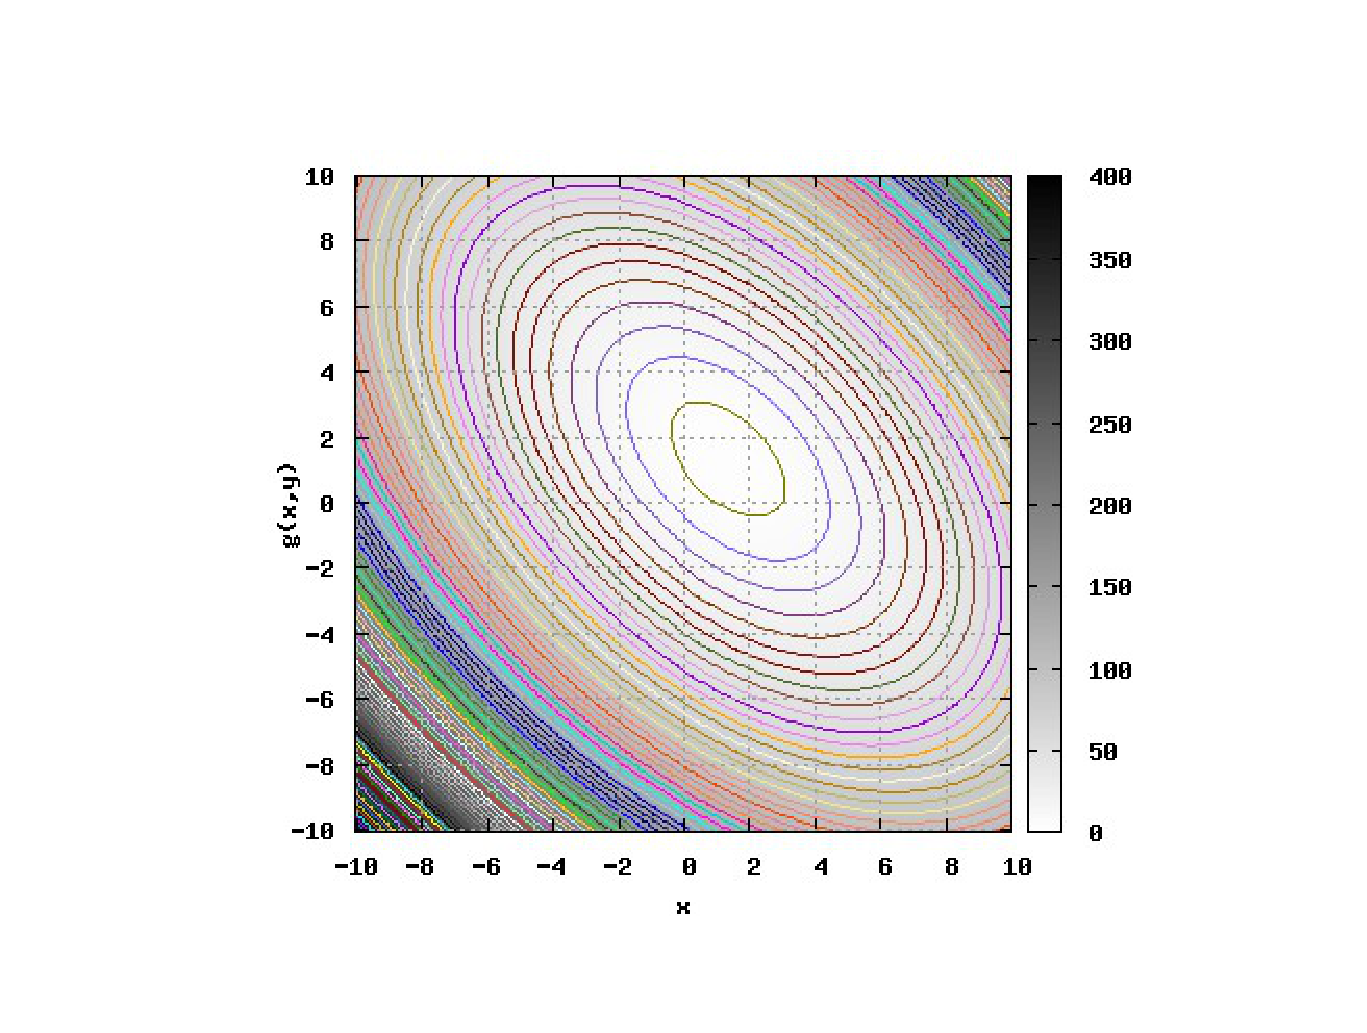
\includegraphics[scale=0.8]{f.eps}
\end{figure}
\end{center}
\item Wnioski\\
Metoda Newtona sprawdza się przy wyznaczaniu miejsc zerowych funkcji dwóch zmiennych.
\end{enumerate}
\end{document}
